% --------------------------------------------------------------
% This is all preamble stuff that you don't have to worry about.
% Head down to where it says "Start here"
% --------------------------------------------------------------
 
\documentclass[12pt]{article}
 
\usepackage{subcaption}
\usepackage[margin=1in]{geometry} 
\usepackage{amsmath,amsthm,amssymb,scrextend}
\usepackage{fancyhdr}
\usepackage{enumitem}
\usepackage{amsmath}
\usepackage{amssymb}
\usepackage{textcomp}
\usepackage{fancybox}
\usepackage{tikz}
\usepackage{tasks}
\pagestyle{fancy}
\usepackage[makeroom]{cancel}
\usepackage{graphicx}
\usepackage{caption}
\usepackage{mwe}
\usepackage{tikz}
\usetikzlibrary{positioning}

\newcommand{\N}{\mathbb{N}}
\newcommand{\Z}{\mathbb{Z}}
\newcommand{\I}{\mathbb{I}}
\newcommand{\R}{\mathbb{R}}
\newcommand{\Q}{\mathbb{Q}}
\renewcommand{\qed}{\hfill$\blacksquare$}
\let\newproof\proof
\renewenvironment{proof}{\begin{addmargin}[1em]{0em}\begin{newproof}}{\end{newproof}\end{addmargin}\qed}
% \newcommand{\expl}[1]{\text{\hfill[#1]}$}
 
\newenvironment{theorem}[2][Theorem]{\begin{trivlist}
\item[\hskip \labelsep {\bfseries #1}\hskip \labelsep {\bfseries #2.}]}{\end{trivlist}}
\newenvironment{lemma}[2][Lemma]{\begin{trivlist}
\item[\hskip \labelsep {\bfseries #1}\hskip \labelsep {\bfseries #2.}]}{\end{trivlist}}
\newenvironment{problem}[2][Problem]{\begin{trivlist}
\item[\hskip \labelsep {\bfseries #1}\hskip \labelsep {\bfseries #2.}]}{\end{trivlist}}
\newenvironment{exercise}[2][Exercise]{\begin{trivlist}
\item[\hskip \labelsep {\bfseries #1}\hskip \labelsep {\bfseries #2.}]}{\end{trivlist}}
\newenvironment{reflection}[2][Reflection]{\begin{trivlist}
\item[\hskip \labelsep {\bfseries #1}\hskip \labelsep {\bfseries #2.}]}{\end{trivlist}}
\newenvironment{proposition}[2][Proposition]{\begin{trivlist}
\item[\hskip \labelsep {\bfseries #1}\hskip \labelsep {\bfseries #2.}]}{\end{trivlist}}
\newenvironment{corollary}[2][Corollary]{\begin{trivlist}
\item[\hskip \labelsep {\bfseries #1}\hskip \labelsep {\bfseries #2.}]}{\end{trivlist}}
 
\setlength{\parindent}{0pt}
\begin{document}
 \settasks{
	counter-format=(tsk[r]),
	label-width=4ex
}
\newcommand\independent{\protect\mathpalette{\protect\independenT}{\perp}}
\def\independenT#1#2{\mathrel{\rlap{$#1#2$}\mkern2mu{#1#2}}}
% --------------------------------------------------------------
%                         Start here
% --------------------------------------------------------------

\lhead{Math 632}
\chead{Continuous Time Markov Chains}
\rhead{Meenmo Kang}

Philosophically exactly like in discrete time: given the present state, the past and the future are independent. But the math becomes more technical. Throughout, the state space $S$ is finite or countably infinite.\\

{\bf Definition} Let $\{X_t:0\le t< \infty\}$ be a stochastic process. Then $X$ is a Markov chain if for all $0\le s_0<\ldots<s_n<s<t$ and all $x_0,\ldots,x_n,x,y\in S:$
$$P(X_t=y\;|\;X_s=x,\;X_{s_n}=x_n,\ldots,X_{s_0}=x_0) = P(X_t=y\;|\;X_s=x)$$ 
wherever the conditioning event has positive probability.

\vspace{1\baselineskip}
We will only deal with the time-homogeneous case where
$$P(X_t=y\;|\;X_s=x) = P(X_{t-s}=y\;|\;X_0=x)$$
The \underline{transition probability} is 
$$P_t^{(x,y)} = P(X_t=y\;|\;X_0=x)$$

Since there are \underline{uncountably} many transition matrices $\{P_t(x,y)\}_{x,y\in S},$ the transition probability is not as useful as in discrete time. It even turns out to be extremely had to calculate in some cases.


\begin{figure}[!htbp]
    \centering
    \begin{subfigure}[b]{0.3\textwidth}
        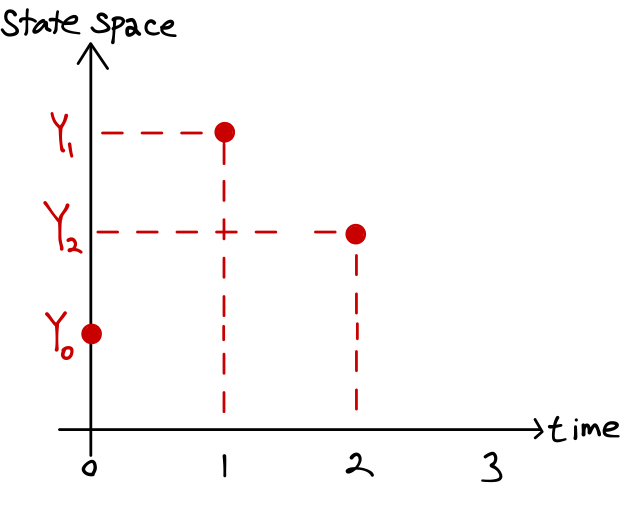
\includegraphics[height=5cm, width=6.5cm]{CTMC_1.jpeg}
        \caption{Discrete-Time MC}
    \end{subfigure}\qquad\qquad
    \begin{subfigure}[b]{0.3\textwidth}
        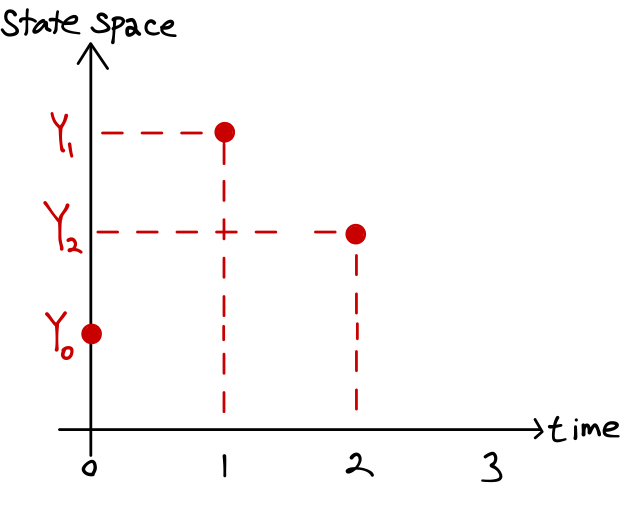
\includegraphics[height=5cm, width=6.5cm]{CTMC_1.jpeg}
        \caption{Continuous-Time MC}
    \end{subfigure}
\end{figure}

The Markov property \underline{force} the holding times $t_1,t_2,t_3,...$ to be exponential random variables. By the same token, the sequence of states visited has to be a discrete-time Markov chain.

\vspace{1\baselineskip}
{\sl Recall the following:}\\
Let $\eta_1,\eta_2,...,\eta_n$ be independent. $\eta\sim\Exp(\lambda)$. $\zeta = \min\{\eta_1,...,\eta_n\}$. I = the index $i$ s.t. $\eta_1 = \zeta$.
$$\zeta \independent I \qquad \zeta\sim\exp(\lambda_1+\ldots+\lambda_n)$$
$$P(\zeta>t)=\prod\limits_{i=1}^n P(\eta_i > t) = \prod\limits_{i=1}^n e^{-\lambda_i t} = e^{-(\lambda_1+\ldots+\lambda_n)t}\qquad\;\;
P(I=1) = \frac{\lambda_i}{\sum\limits_{j=1}^n \lambda_j}$$

\newpage
{\bf Special case} Let $(Y_n)$ be a discrete-time Markov chain with transition matrix $u=(u(x,y))_{x,y\in S}$. Let $N(t)$ be a rate $\lambda$ Poisson process. Then $X_t = Y_{N(t)}$ is a continuous time Markov chain.

In this {\bf SPECIAL CASE} we can calculate the transition probability:
\begin{align}
    P_t(x,y) &= P(x_t=y\;|\;X_0=x) = P(X_t=y\;|\;Y_0=x) \nonumber \\
    &=\sum\limits_{n=0}^\infty P(X_t=y,\;N(t)=n\;|\;Y_0=x) \nonumber \\
    &\text{\quad (N(t): the number of jumps by time t)} \nonumber \\
    &=\sum\limits_{n=0}^\infty P(Y_n=y,\;N(t)=n\;|\;Y_0=x) \nonumber \\ 
    &=\sum\limits_{n=0}^\infty P(N(t)=n)P(Y_n=y\;|\;Y_0=x) \nonumber \\
    &= \sum\limits_{n=0}^\infty \frac{e^{-\lambda t} (\lambda t)^n}{n!} \cdot u^n(x,y) \nonumber
\end{align}

Note that $Z\sim$ Poisson($\mu$) then
$$P(Z=k) = \frac{e^{-\mu}\mu^k}{k!}$$

\vspace{1\baselineskip}
What takes the place of the transition probabilities as the fundamental object? {\bf Rates}.\\

{\bf Definition} For $x\neq y$ in $S$, the \underline{Rate} of jumping from $x$ to $y$ is 
$$q(x,y)=\lim\limits_{h\to 0} \frac{P_h(x,y)}{h}$$
This limit will exist in all our examples. \\

\vspace{1\baselineskip}
Note that 
$$u^{(0)}(x,y) = \begin{cases} 1&x=y\\0&x\neq y\end{cases}$$
$$u^{(0)} = I = \text{the identity matrix}$$

\vspace{1\baselineskip}
Back to the previous {\bf SPECIAL CASE:}
\begin{align}
    \frac{1}{h}p_h(x,y) &= \frac{1}{h} \sum\limits_{n=0}^\infty \frac{e^{\lambda h}(\lambda h)^n}{n!} u^n(x,y) \nonumber \\
    \text{n=0\; term = 0!} \nonumber \\
    &=\underbrace{0}_{n=0} \underbrace{e^{-\lambda h}\lambda u(x,y)}_{n=1} + \underbrace{\frac{1}{h} \sum\limits_{n=2}^\infty \frac{\overbrace{e^{-\lambda h}}^{=1}(\lambda h)^n}{n!} \overbrace{u^{(n)}(x,y)}^{=1}}_{0\le \cdot \le \frac{1}{h}h^2\sum\limits_{n=2}^\infty \frac{}}
\end{align}
INCOMPLETE

\vspace{1\baselineskip}
So $q(x,y)=\lambda u(x,y)$ where $\lambda$ is the rate of Poisson clock and $u(x,y)$ is the probability of jumping to $y$.

\vspace{1\baselineskip}
"little oh of h" o(h) means a quantity that when divided by $h$ goes to o as $h\to 0,\;\frac{o(h)}{h}\xrightarrow{h\to 0} 0$

\vspace{1\baselineskip}
\rightarrow Hence forth we will give our examples in terms of rates.

\vspace{1\baselineskip}
{\sl Ex.} Let $N(\cdot)$ be a rate $\lambda$ Poisson process. Then $N(\cdot)$ is a Markov chain with stable space $S=Z_{\ge 0}$ and rates
\end{document}